\documentclass[11pt]{article}
\usepackage[margin=1in]{geometry}
\usepackage{graphicx}
\usepackage{booktabs}
\usepackage{array}
\usepackage{float}
\usepackage{hyperref}

\setlength{\parindent}{0pt}
\setlength{\parskip}{0.5em}

\title{Final Report\\\textbf{Detecting and Mitigating Simple IoT-Based DoS Attacks}}
\author{Group 8}
\date{\today}

\begin{document}
\maketitle

\section*{Abstract}
Internet of Things (IoT) devices are now used in many places, but many of them still have weak
security. Because of this, compromised IoT devices can be used to launch denial-of-service (DoS)
attacks. In this project, we build a lightweight and explainable system to detect simple IoT-based
DoS attacks from simulated traffic traces. The system uses rule-based detection with packet-level
features such as packet rate, byte rate, SYN count, and destination-port diversity. We evaluate
adaptive, fixed, hybrid, and hybrid-persistent threshold strategies over 10 random seeds. The
result shows that the hybrid-persistent detector gives the best practical balance in our
experiment. It improves the tradeoff between attack detection and false positives better than the
pure adaptive and fixed detectors, even though UDP-flood detection is still limited.

\section*{Introduction}
IoT devices are becoming common in home networks, campus networks, and enterprise systems. Many
of these devices are low-cost and resource-limited, so strong security protection is not always
included. Because of this situation, IoT devices can be compromised and used in DoS attacks. Such
attacks can reduce service availability and create serious network problems.

Many research works on IoT security use complex machine learning models or large testbeds. These
methods are useful, but they are not always easy to reproduce in a classroom environment. In this
project, we wanted to study a simpler approach. Our goal was to build a lightweight detector that
is easy to explain, easy to run, and still meaningful for network security study.

\section*{Problem Statement and Objectives}
The main problem in this project is to distinguish normal IoT traffic from attack traffic using
simple traffic behavior in short time windows. We focus on a rule-based detector instead of a
machine learning detector because the main interest of this work is explainability and practical
implementation for a course project.

The objectives of the project are:
\begin{itemize}
  \item generate normal and attack traffic for a small IoT scenario,
  \item extract lightweight traffic features from packet traces,
  \item detect suspicious traffic using threshold-based rules,
  \item compare several detector configurations,
  \item evaluate the result with multiple seeds and visual summaries.
\end{itemize}

\section*{System Design}
The system is implemented as a small Python pipeline. Each script has one main responsibility in
the workflow.

\begin{itemize}
  \item \texttt{traffic\_generator.py} generates synthetic traffic and writes labeled PCAP data.
  \item \texttt{feature\_extractor.py} reads the PCAP and computes per-second features.
  \item \texttt{detector.py} applies the threshold-based detection logic.
  \item \texttt{evaluator.py} computes metrics and phase-level summaries.
  \item \texttt{visualizer.py} produces figures for analysis.
  \item \texttt{main.py} runs the complete pipeline and experiment loop.
\end{itemize}

This modular design makes the project easier to test, modify, and explain.

\section*{Methodology}
The traffic model contains four main behavior types: normal traffic, benign burst traffic, UDP
flood traffic, and TCP SYN flood traffic. The benign burst phase is important because it represents
a legitimate sudden increase in traffic, such as a firmware update. This helps us evaluate false
positives, not only attack detection.

Traffic is divided into one-second windows. For each window, the system computes these features:
\begin{itemize}
  \item packets per second,
  \item bytes per second,
  \item SYN packets per second,
  \item number of unique destination ports,
  \item number of unique destination IPs.
\end{itemize}

We compare four rule-based detector configurations:
\begin{itemize}
  \item \textbf{Adaptive:} rolling baseline mean + standard deviation threshold,
  \item \textbf{Fixed:} threshold from initial calibration period,
  \item \textbf{Hybrid:} adaptive threshold for UDP-style features and fixed threshold for SYN-style features,
  \item \textbf{Hybrid-persistent:} hybrid detector with two consecutive suspicious windows required before alert.
\end{itemize}

The rule logic is also simple and explainable. UDP-flood style behavior is flagged when packet
rate and byte rate are both high. SYN-flood style behavior is flagged when SYN count and
destination-port diversity are both high. We also use a simulated mitigation step, where the
system records a block or rate-limit action in a log file.

\section*{Experimental Setup}
All experiments are based on synthetic traffic traces generated with Python and Scapy. The data is
evaluated offline from PCAP files. We use 10 random seeds to reduce the chance that the result is
coming from one special run only. The benign burst intensity is slightly varied across seeds so the
evaluation is a little more realistic.

The final comparison uses averaged metrics across these 10 seeds. We report accuracy, precision,
recall, false positive rate (FPR), F1 score, firmware-burst false positive rate, UDP recall, and
SYN recall. We also include a feature ablation study to show how different feature subsets affect
the result.

\section*{Results}
Table~\ref{tab:maincomparison} is the main detector comparison in this project. It shows clearly
that the adaptive detector is too conservative, while the fixed detector is too aggressive during
the benign burst phase. The hybrid and hybrid-persistent detectors give a better balance.

\begin{table}[H]
\centering
\caption{Main detector comparison averaged over 10 seeds}
\label{tab:maincomparison}
\begin{tabular}{>{\raggedright\arraybackslash}p{2.8cm}cccccccc}
\toprule
\textbf{Detector} & \textbf{Accuracy} & \textbf{Precision} & \textbf{Recall} & \textbf{FPR} & \textbf{F1} & \textbf{Burst FPR} & \textbf{UDP Recall} & \textbf{SYN Recall} \\
\midrule
Adaptive & 0.7644 & 0.6264 & 0.1400 & 0.0275 & 0.2286 & 0.3300 & 0.1250 & 0.1550 \\
Fixed & 0.9375 & 0.8000 & 1.0000 & 0.0833 & 0.8889 & 1.0000 & 1.0000 & 1.0000 \\
Hybrid & 0.8700 & 0.8721 & 0.5625 & 0.0275 & 0.6837 & 0.3300 & 0.1250 & 1.0000 \\
Hybrid-persistent & 0.8713 & 0.8919 & 0.5525 & 0.0225 & 0.6821 & 0.2700 & 0.1050 & 1.0000 \\
\bottomrule
\end{tabular}
\end{table}

Table~\ref{tab:maincomparison} shows that the fixed detector has the highest recall, but it also
flags all benign burst windows as attack. Because of this, it is not the most practical choice.
The hybrid-persistent detector gives a better balance. It reduces firmware-burst false positive
rate from 0.33 in the plain hybrid detector to 0.27, and it also keeps the lowest overall false
positive rate among the stronger detectors.

\begin{figure}[H]
  \centering
  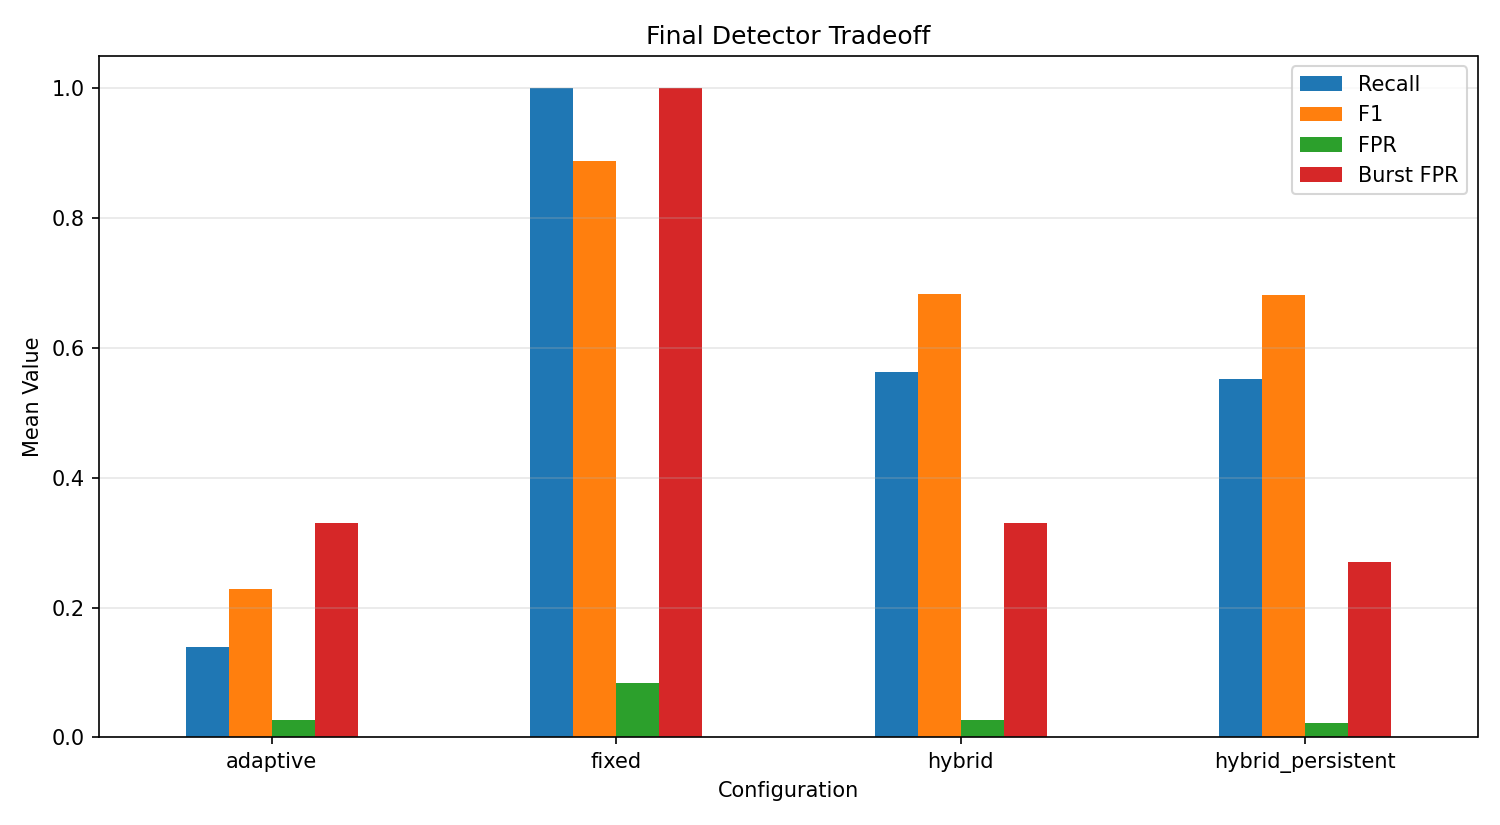
\includegraphics[width=0.9\linewidth]{figures/final_tradeoff_bars.png}
  \caption{This final-only figure compares the most important final metrics together. It helps show why hybrid-persistent gives the most balanced result when recall, F1, overall false positive rate, and burst false positive rate are considered together.}
  \label{fig:tradeoff}
\end{figure}

Figure~\ref{fig:tradeoff} is a new figure for the final report. It is stronger than the older
recall-only figure because it compares the most important values side by side. The fixed detector
is strong in recall and F1, but it is not attractive because both false positive measures are
high. The hybrid-persistent detector keeps strong recall and F1 while lowering false positive
behavior compared with the other practical choices, so this supports our final choice.

\begin{figure}[H]
  \centering
  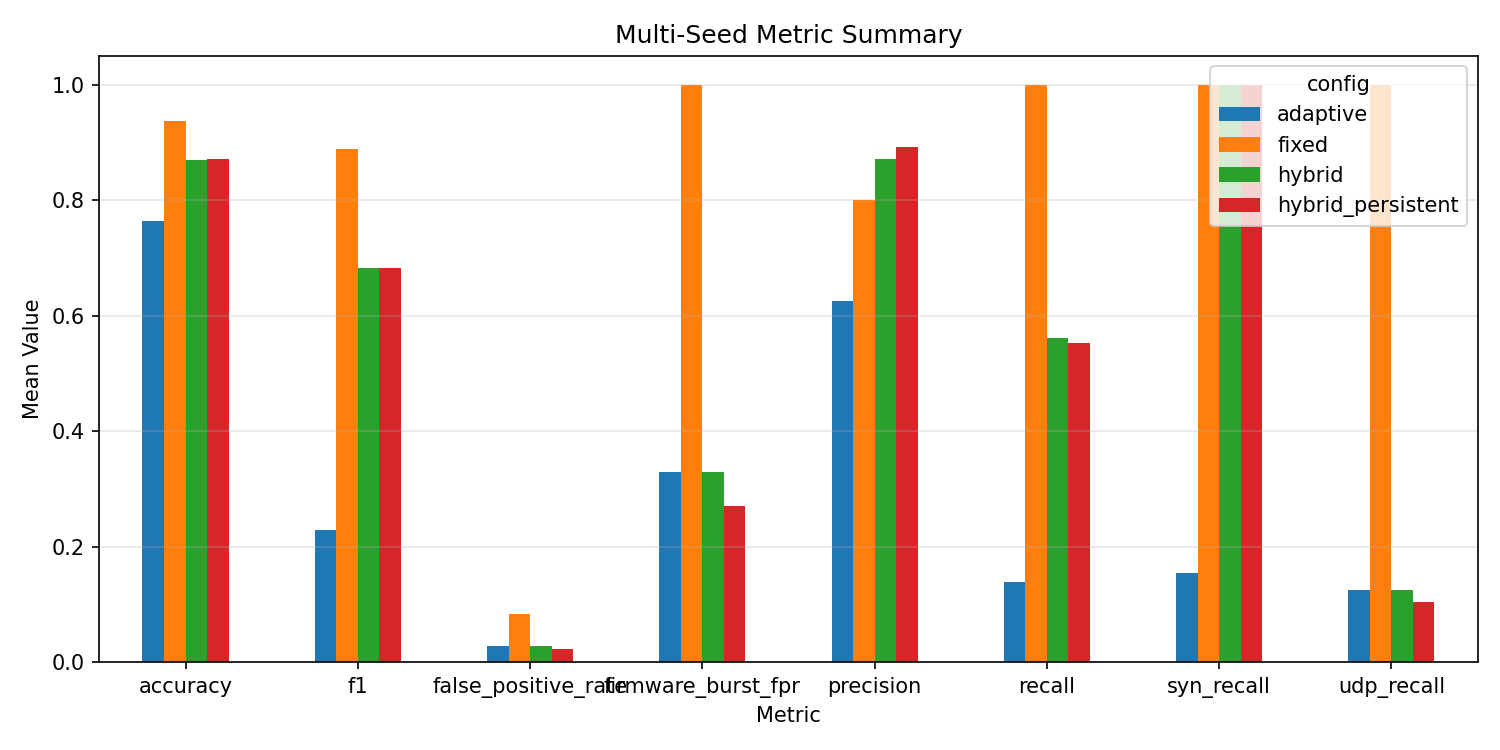
\includegraphics[width=\linewidth]{figures/multi_seed_summary.png}
  \caption{This figure shows the tradeoff across multiple evaluation metrics, not only recall, so it makes the comparison more credible.}
  \label{fig:multiseed}
\end{figure}

Figure~\ref{fig:multiseed} is useful because it shows several metrics together. The fixed detector
looks very strong in recall and F1, but it also has the worst burst false positive behavior. The
hybrid-persistent detector does not give the highest recall, but it gives a more balanced
performance when we consider multiple metrics together.

\begin{figure}[H]
  \centering
  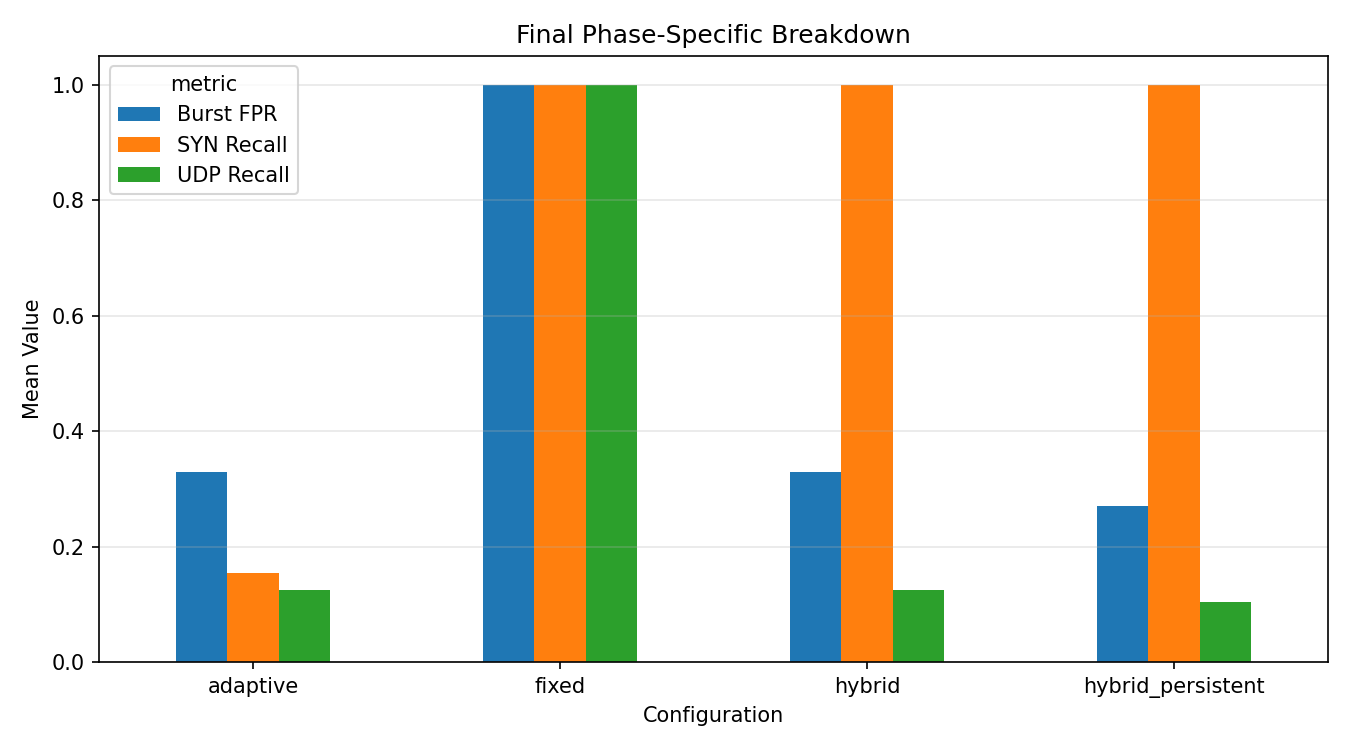
\includegraphics[width=0.9\linewidth]{figures/final_phase_breakdown.png}
  \caption{This final-only figure focuses on the three most important final metrics: firmware-burst false positive rate, UDP recall, and SYN recall. It makes the final configuration choice easier to justify.}
  \label{fig:phasebreakdown}
\end{figure}

Figure~\ref{fig:phasebreakdown} is also a new figure for the final report. It shows more clearly
why the final detector decision is not only about overall recall. The fixed detector detects both
attack types very strongly, but it also has the worst burst false positive rate. The
hybrid-persistent detector lowers the burst false positives compared with hybrid and still keeps
perfect SYN recall.

\begin{table}[H]
\centering
\caption{Feature ablation results for the adaptive detector}
\label{tab:ablation}
\begin{tabular}{>{\raggedright\arraybackslash}p{3.2cm}ccccc}
\toprule
\textbf{Feature Set} & \textbf{Accuracy} & \textbf{Precision} & \textbf{Recall} & \textbf{FPR} & \textbf{F1} \\
\midrule
Packets only & 0.7506 & 0.5071 & 0.0875 & 0.0283 & 0.1491 \\
Packets + bytes & 0.7450 & 0.4233 & 0.0625 & 0.0275 & 0.1087 \\
SYN + ports & 0.7694 & 1.0000 & 0.0775 & 0.0000 & 0.1436 \\
Full feature set & 0.7644 & 0.6264 & 0.1400 & 0.0275 & 0.2286 \\
\bottomrule
\end{tabular}
\end{table}

Table~\ref{tab:ablation} shows that the full feature set gives the best overall recall and F1
score for the adaptive detector. The SYN + ports feature set has perfect precision, but it misses
many attack windows. This result suggests that SYN-flood behavior is easier to detect with simple
features, but UDP-flood behavior still needs more help from combined features.

\begin{figure}[H]
  \centering
  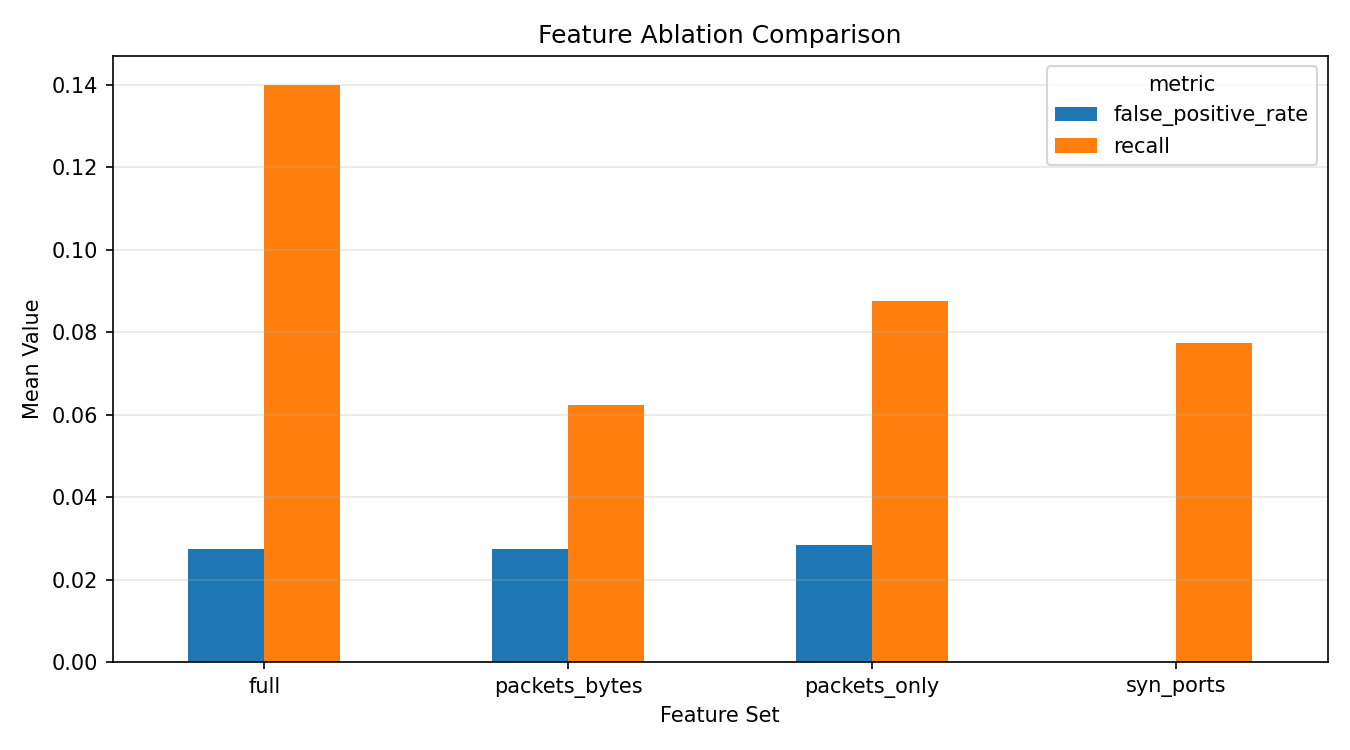
\includegraphics[width=0.82\linewidth]{figures/ablation_comparison.png}
  \caption{This figure supports that feature choice matters, and the full feature set gives the most balanced result for the adaptive detector.}
  \label{fig:ablation}
\end{figure}

Figure~\ref{fig:ablation} makes the ablation result easier to understand. The simple subsets are
not enough to give both good recall and controlled false positives. The full feature set is still
the most useful choice in this project.

\begin{table}[H]
\centering
\caption{Important phase-level interpretation for the hybrid-persistent detector}
\label{tab:phase}
\begin{tabular}{>{\raggedright\arraybackslash}p{2.8cm}>{\raggedright\arraybackslash}p{1.6cm}c>{\raggedright\arraybackslash}p{6.4cm}}
\toprule
\textbf{Phase} & \textbf{Type} & \textbf{Rate} & \textbf{Interpretation} \\
\midrule
Firmware burst & Benign & FPR = 0.27 & Some burst windows are still flagged, so benign spikes are still difficult for the detector. \\
Normal\_1 & Benign & FPR = 0.00 & Regular normal traffic is handled correctly. \\
UDP flood & Attack & Recall = 0.105 & UDP flood is still hard to detect well with the current simple rule-based method. \\
SYN flood & Attack & Recall = 1.00 & SYN flood is detected very well by the final detector. \\
\bottomrule
\end{tabular}
\end{table}

Table~\ref{tab:phase} helps explain where the final detector is strong and where it is weak. The
main weakness is still UDP-flood detection. On the other hand, normal traffic is mostly handled
correctly, and SYN flood detection is very strong.

\begin{figure}[H]
  \centering
  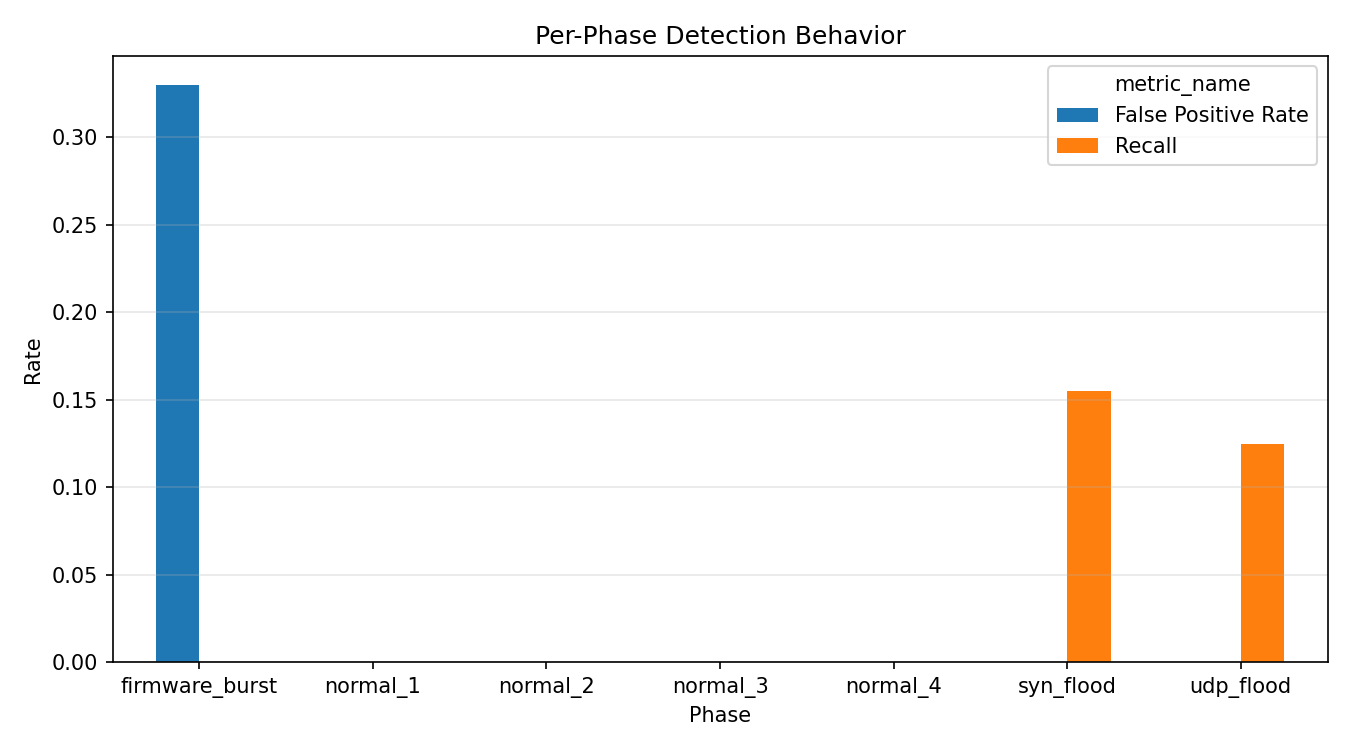
\includegraphics[width=0.88\linewidth]{figures/phase_metrics.png}
  \caption{This figure shows that benign burst traffic is the most difficult normal phase, while attack behavior is not equally easy for UDP flood and SYN flood.}
  \label{fig:phase}
\end{figure}

Figure~\ref{fig:phase} gives a phase-level explanation for the final detector behavior. It shows
that the burst phase is the most confusing benign phase, and it also shows that the two attack
types do not have the same difficulty. This supports the claim that UDP flood remains the weaker
part of the final system.

\section*{Discussion}
Based on the final experiment, we consider the hybrid-persistent detector as the best practical
choice in this project. It does not give the highest recall, but it gives a more balanced tradeoff
between false positives and attack detection. This is important because a detector with many false
alarms is not practical in a real environment.

The adaptive detector is too conservative. It keeps false positives lower, but it misses too many
attack windows. The fixed detector is the opposite case. It catches attacks very strongly, but it
also treats the benign burst as attack almost all the time. The hybrid detector improves the
balance, and the persistence rule makes it slightly better again by reducing unstable alerting.

One important observation is that SYN-flood traffic is much easier to detect than UDP-flood
traffic in our setup. This is because SYN flood has a stronger and cleaner feature pattern, mainly
in SYN count and destination-port diversity. UDP flood is harder because some of its behavior can
look more similar to a sudden but normal burst.

\section*{Limitations}
This project has several limitations. First, the traffic is synthetic, so it does not include all
the noise and unpredictability of real IoT networks. Second, the mitigation stage is only
simulated, so we do not test a real firewall or real deployment behavior. Third, the final system
still has low UDP recall, which means the detector is not equally strong for all DoS types.

Another limitation is that the project uses a small and controlled environment. This is useful for
reproducibility, but it also means the result should be interpreted as a course-scale prototype
and not as a complete production security system.

\section*{Conclusion}
In this project, we designed and evaluated a lightweight and explainable IoT-based DoS detection
system using simulated traffic. The project shows that simple threshold logic can be useful,
especially when the detector is carefully designed and compared with multiple configurations.

The final result shows that hybrid-persistent detection gives the best practical balance in our
experiment. It does not solve every problem, and UDP flood is still difficult, but the system is
simple, understandable, and reproducible. For a course project, this is a useful result because it
shows how basic traffic analysis can still provide meaningful security insight without requiring a
very complex infrastructure.

\end{document}
